\section{Results}
I have calculated binding energies with and without the independent pair correlations and compared the results. In both cases we have used the v6 potential and the same operators for the correlations. In each case the weights for each operator was determined variationally. Calculations were done for systems, $^4$He and $^{16}$O and the binding energies are reported in table \ref{tab:indpairresults} with and without independent pairs correlations and compared to the experimental value.

\begin{table}[h!]
   \centering
   \caption{Binding energies in MeV for $^4$He and $^{16}$O as calculated with and without independent pair correlations (IPC) compared to experimental energies.}
   \label{tab:indpairresults}
   \begin{tabular}{ccccc}
      \hline \hline
%       & Without IPC & With IPC & Expt.\\
       & Linear & IndPair & Quadratic & Expt.\\
      \hline
      $^4$He & -27.0(3) & -26.3(3) & -28.5(2) & -28.295\\
      $^{16}$O & -114(3) & -132(3) & -143.3(3) & -127.619\\
      \hline \hline
   \end{tabular}
\end{table}

I have also calculated the binding energy per nucleon of symmetric nuclear matter with density $\rho=0.16$fm$^{-1}$ of 28 particles with periodic boundary conditions. The energy per nucleon was -14.3(2) MeV without the independent pair correlations and -16.6(2) MeV with the independent pair correlations.

\begin{figure}[h!]
   \centering
   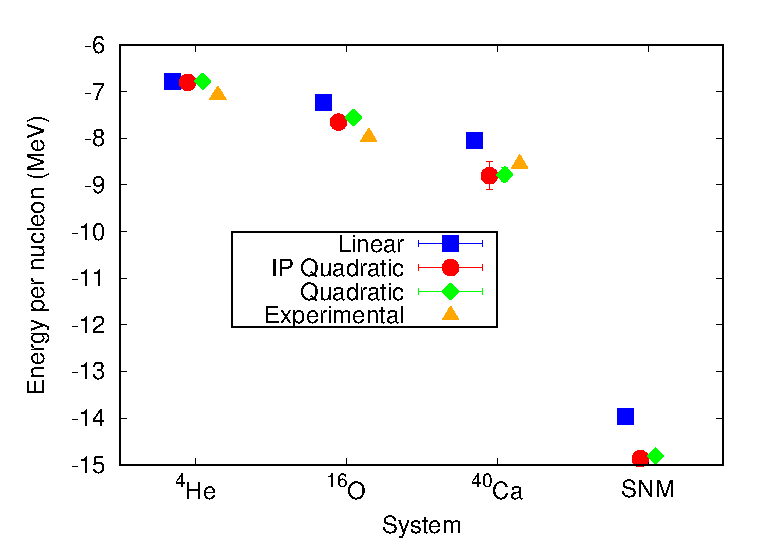
\includegraphics[width=0.5\textwidth]{energies.eps}
   \caption{Binding energies for ${}^4$He and ${}^{16}$O as calculated with linear, independent pair, and quadratic correlations. Also, the energy per nucleon of symmetric nuclear matter as calculated from 28 particles in a periodic box. All calculations are compared to their expected values.}
   \label{fig:energies}
\end{figure}
